\documentclass[a4paper,10pt]{article}
\usepackage{amsmath,amsfonts,amsthm,amssymb,fullpage,enumerate}
\usepackage{pgf,tikz,tikz-cd}
\usepackage{graphicx}
\usepackage{setspace}
\usepackage{epstopdf}
\usepackage{mathrsfs}
\usepackage{cite}
\usepackage{hyperref,url}
\usepackage{algorithm}
\usepackage{ulem}
\usepackage[noend]{algpseudocode}
\usepackage{MnSymbol}
\newcommand{\CC}{\mathbb{C}}
\newcommand{\RR}{\mathbb{R}}
\newcommand{\NN}{\mathbb{N}}
\newcommand{\QQ}{\mathbb{Q}}
\newcommand{\ZZ}{\mathbb{Z}}
\newcommand{\TS}{\mathcal{T}}
\newcommand{\EE}{\mathbb{E}}
\newcommand{\FF}{\mathbb{F}}
\newcommand{\GG}{\mathcal{G}}
\newcommand{\PP}{\mathbb{P}}
\newcommand{\BB}{\mathcal{B}}
\newcommand{\dd}{\,\mathrm{d}}
\newcommand{\II}{\mathbb{I}}
\newcommand{\ul}{\underline}
\newcommand{\zero}{\{0\}}			
\newcommand{\va}{\mathbf{a}}
\newcommand{\Var}{\text{Var}}
\newcommand{\vx}{\mathbf{x}}
\providecommand{\norm}[1]{\|\cdot\|_{#1}}
\providecommand{\normm}[2]{\left\|{#1}\right\|_{#2}}
\providecommand{\ip}[1]{\bds\left( #1 \right)\eds}
\DeclareMathOperator{\interior}{int}
\DeclareMathOperator{\exterior}{ext}
\newtheorem{thm}{Theorem}
\newtheorem{Def}[thm]{Definition}
\newtheorem{Cor}[thm]{Corollary}
\newtheorem{cl}[thm]{Claim}
\newtheorem{prop}[thm]{Proposition}
\newtheorem{eg}[thm]{Example}
\newtheorem{Ex}[thm]{Exercise}
\newtheorem{Lem}[thm]{Lemma}
\newtheorem{note}[thm]{Note}
\newtheorem{rem}[thm]{Remark}
\newcommand{\bds}{\begin{displaystyle}}
\newcommand{\eds}{\end{displaystyle}}
\newcommand{\bpm}{\begin{pmatrix}}
\newcommand{\epm}{\end{pmatrix}}
\newcommand{\bvm}{\begin{vmatrix}}
\newcommand{\evm}{\end{vmatrix}}
\newcommand{\conj}{\overline}
\newcommand{\inv}{^{-1}}
\newcommand{\Ito}{It$\hat{\text{o}}$} 
\newcommand{\cadlag}{\textit{c\`{a}dl\`{a}g}}
\newcommand{\Cadlag}{\textit{C\`{a}dl\`{a}g}}
\newcommand{\Cech}{\v{C}ech}
\newcommand{\Frechet}{Frech\`{e}t}

\newcommand{\im}{\text{im}}

\makeatletter
\newcommand{\chaptersubheading}[1]{%
  {\parindent0pt\vspace*{-25pt}%
  \linespread{1.1}\large\scshape#1%
  \par\nobreak\vspace*{35pt}}
  \@afterheading%
}
\makeatother




\usepackage{xcolor}
\def\cblu{\color{blue}}
\def\cred{\color{red}}
\def\cgre{\color{green}}

\setlength{\parindent}{0pt}
\numberwithin{equation}{section}
\numberwithin{thm}{section}


\begin{document}

\title{Posterior Sampling with Proximal MCMC}
\author{Louis Christie \\ \href{mailto:lgc26@cam.ac.uk}{\textit{lgc26@cam.ac.uk}} }
\maketitle

\doublespacing


\section{Introduction}

In many image settings we are interested in the inverse problem of finding $x \in \mathbb{X}$ when we see $y \sim N( Ax, V )$ for example. One way to do this is to find a posterior distribution 
\begin{equation}
\label{eq:posterior}
\pi_{X \mid Y} (x \mid y ) \propto \pi_{Y \mid X } ( y \mid x ) \times \pi_X (x) = N( y \mid Ax, V) \times \pi_X(x)
\end{equation}
This requires us to specify a prior $\pi_X(x)$, which is often done by training a neural network or other model on a set of accurate images. \\
\\
Once we've specified the prior and likelihood, we can estimate $x$ from the posterior. One way is to find the Maximum A Posteriori (MAP) estimate $\hat{x}^{MAP} = \arg \max_{u \in \mathbb{X} } \pi_{X \mid Y}(u \mid y)$. Another is to find the posterior expectation $\hat{x} = \EE( X \mid y )$. Since it may not be possible to analytically find this expectation, we turn to Monte-Carlo integration:
\begin{equation}
 \EE( X \mid Y ) \approx \frac{1}{m} \sum_{i = 1}^m X_i \qquad \text{where } X_i \overset{iid}{\sim} \pi_{X \mid Y}
\end{equation}
To do this we need to sample from the posterior, which we do by designing a Markov Chain with the target posterior as its stationary distribution. This also has the benefit of allowing us to quantify the uncertainty in our estimate using the sample variance of these samples. In our case we can use the MYULA chain

\begin{prop}
If $- \log \pi_{X \mid Y} = f + g $ where $f$ is convex, proper, lower semicontinuous and has $L_f$-Lipschitz gradient and $g$ is convex, proper and lower semicontinuous, then the chain with transitions:
\begin{equation}
\label{eq:MYULA}
X_{n+1} = X_n - \delta \nabla f(X_n) - \tfrac{\delta}{\lambda} ( X_n - \text{Prox}_g^\lambda (X_n) ) + \sqrt{2 \delta} Z_{n+1} \tag{MYULA}
\end{equation}
(where $Z_i \overset{iid}{\sim} N(0,\mathbf{1})$ and $\delta < 2 \lambda ( L_f \lambda + 1)^{-1}$) converges exponentially fast to $\pi_{X \mid Y}$ as $n \rightarrow \infty$.
\end{prop}
From equation \ref{eq:posterior} we see that for some normalisation constant $C$:
\begin{equation}
- \log \pi_{X \mid Y} = - \log C - \log \pi_{Y \mid X} - \log \pi_X	
\end{equation}
So we can set $f = - \log C - \log \pi_{Y \mid X}$ and $g = - \log \pi_X$ to use MYULA. This requires computing $\text{Prox}_g^\lambda(X_n) = \arg\min_{u \in \mathbb{X} } ( g(u) + (2\lambda)^{-1} \| x - u \|_\mathbb{X}^2 )$ at each step. This is a strongly convex function so does have a unique minimiser, but we would like to compute it without a descent style algorithm. The question becomes can we learn a prior $\pi_X$ such that this proximal operator can be computed analytically? \\
\\
Since $g$ is sub-differentiable, we can define see that the proximal operator can be rewritten as an inverse image:
\begin{equation}
\text{Prox}_g^\lambda (x) = ( I_\mathbb{X} + \lambda \partial g )^{-1} ( \{x \} )	
\end{equation}
This can be seen as if $u \in (I_\mathbb{X} + \lambda \partial g)(x)$ then $0 \in \lambda \partial g (u) + u - x$ so $u$ is a minimiser of $g(u) + \| x - u \|^2_\mathbb{X} / (2 \lambda)$. Since this is strongly convex, the inverse image is a singleton. \\
\\
{\cred cite Subhadip} have shown that they can learn $g$ as an \textbf{input convex neural network} (ICNN) by using nodes of the form:
\[ z_{i+1} = \phi_i ( B_i (z_i) + W_i(x_i) + b_i) \]
If the weights $B_i$ are all non-negative and the $\phi_i$ are each convex and monotone then the learned network is also convex. \\
\\
If we use a smooth activation function $\phi_i$, this is also guaranteed to be smooth. This means that we can ignore the proximal step in MYULA entirely - we can just use the smooth posterior to sample easily. 


\newpage
\section{Gaussian Example}

Suppose that $A$ is the identity operator, so $y \mid x \sim N( x , \Sigma_\epsilon )$. If we take a Gaussian prior on $X$, so $\pi_X (x) = N( x \mid 0, \Sigma_X)$, then we have a known posterior:
\begin{align}
\pi_{X \mid Y}( x \mid y ) &\propto N( x \mid y , \Sigma_\epsilon ) \times N( x \mid 0, \Sigma_X ) \\
&\propto N( x \mid S ( \Sigma_\epsilon^{-1} y ) 	, S )
\end{align}
where $S^{-1} = \Sigma_\epsilon^{-1} + \Sigma_X^{-1}$. 
\begin{eg}
In Willem's example, we have $y = (1,1)$, $\Sigma_\epsilon = \tfrac{1}{2} I_2$, and $\Sigma_X = I_2$. Thus we have the posterior 
\begin{equation}
	\pi_{X \mid Y}( x \mid (1,1)^T ) = N \bigg( x \ \Big \mid \ \bigg( \begin{smallmatrix} \tfrac{3}{2} \\ \tfrac{3}{2} \end{smallmatrix} \bigg) , \bigg( \begin{smallmatrix} \tfrac{1}{3} & 0 \\ 0 & \tfrac{1}{3} \end{smallmatrix} \bigg) \bigg) 
\end{equation}
Sampling 4000 steps of MYULA with 1000 to burn in gives a sample with a KDE given in figure \ref{fig:gaussian_eg}.
\begin{figure}[h]
\label{fig:gaussian_eg}
\centering
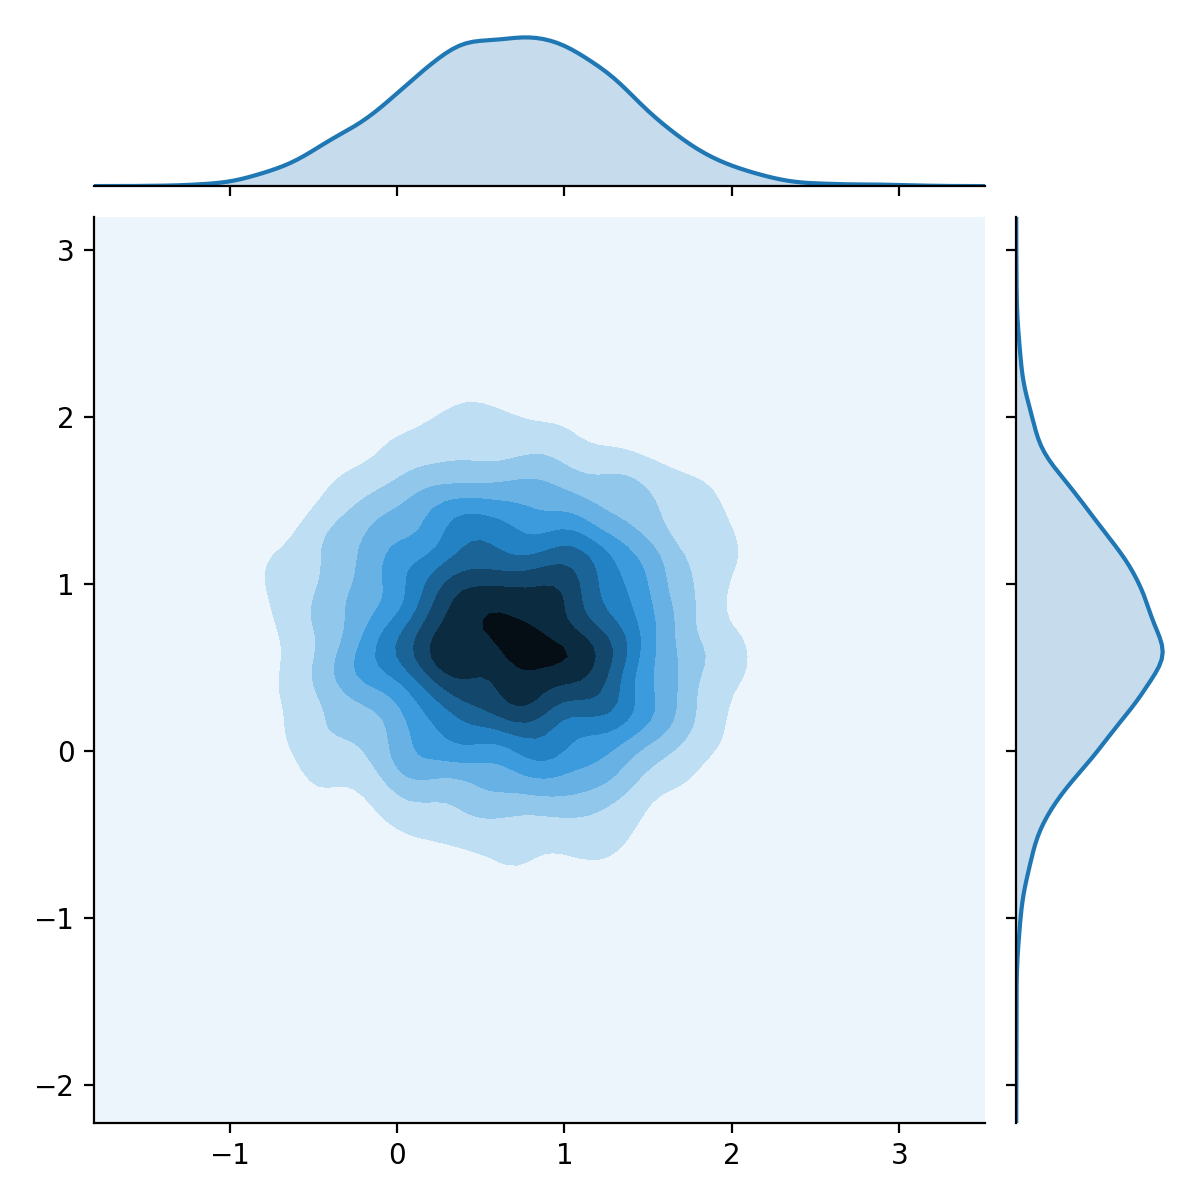
\includegraphics[scale=0.6]{figs/gaussian_eg_posterior.png}	
\caption{Posterior Sample KDE from MYULA. Sample mean at $(0.682, 0.681)^T$ with marginal variances of $0.42$ and $0.38$} 
\end{figure}

\end{eg}


\newpage
\section{Lasso Prior}

In the same context as above we have the likelihood $N( y \mid A x, \Sigma_\epsilon)$, but know we have $- \log \pi_X (x) = g(x) = \| x \|_1$. Thus the prox of $g$ is given by:
\begin{align}
 \text{Prox}_g^\lambda (x) &= \arg \min_{u \in \RR^d} \tfrac{1}{2} \| u - x \|_2^2 + \lambda \|u \|_1
\end{align}
As the objective is separable component wise; we get:
\begin{align}
 \text{Prox}_g^\lambda (x)_i &= \arg \min_{u_i \in \RR} \tfrac{1}{2} ( u_i - x_i )^2 + \lambda |u_i| \\
 	&= \{ u_i \in \RR : 0 \in \partial  \tfrac{1}{2} ( u_i - x_i )^2 + \lambda |u_i| \} \\
 	&= \{ u_i \in \RR : 0 \in (u_i - x_i) + \lambda \text{sign}(u_i) \mathbf{1}_{u_i \neq 0} + \lambda \mathbf{1}_{u_i = 0} [-1,1] \} \\
 	&= \text{sign}(x_i) \max(0, |x_i| - \lambda)
\end{align}
This is called the \textbf{soft-thresholding operator}. 

\begin{figure}[h]
\label{fig:lasso_eg}
\centering
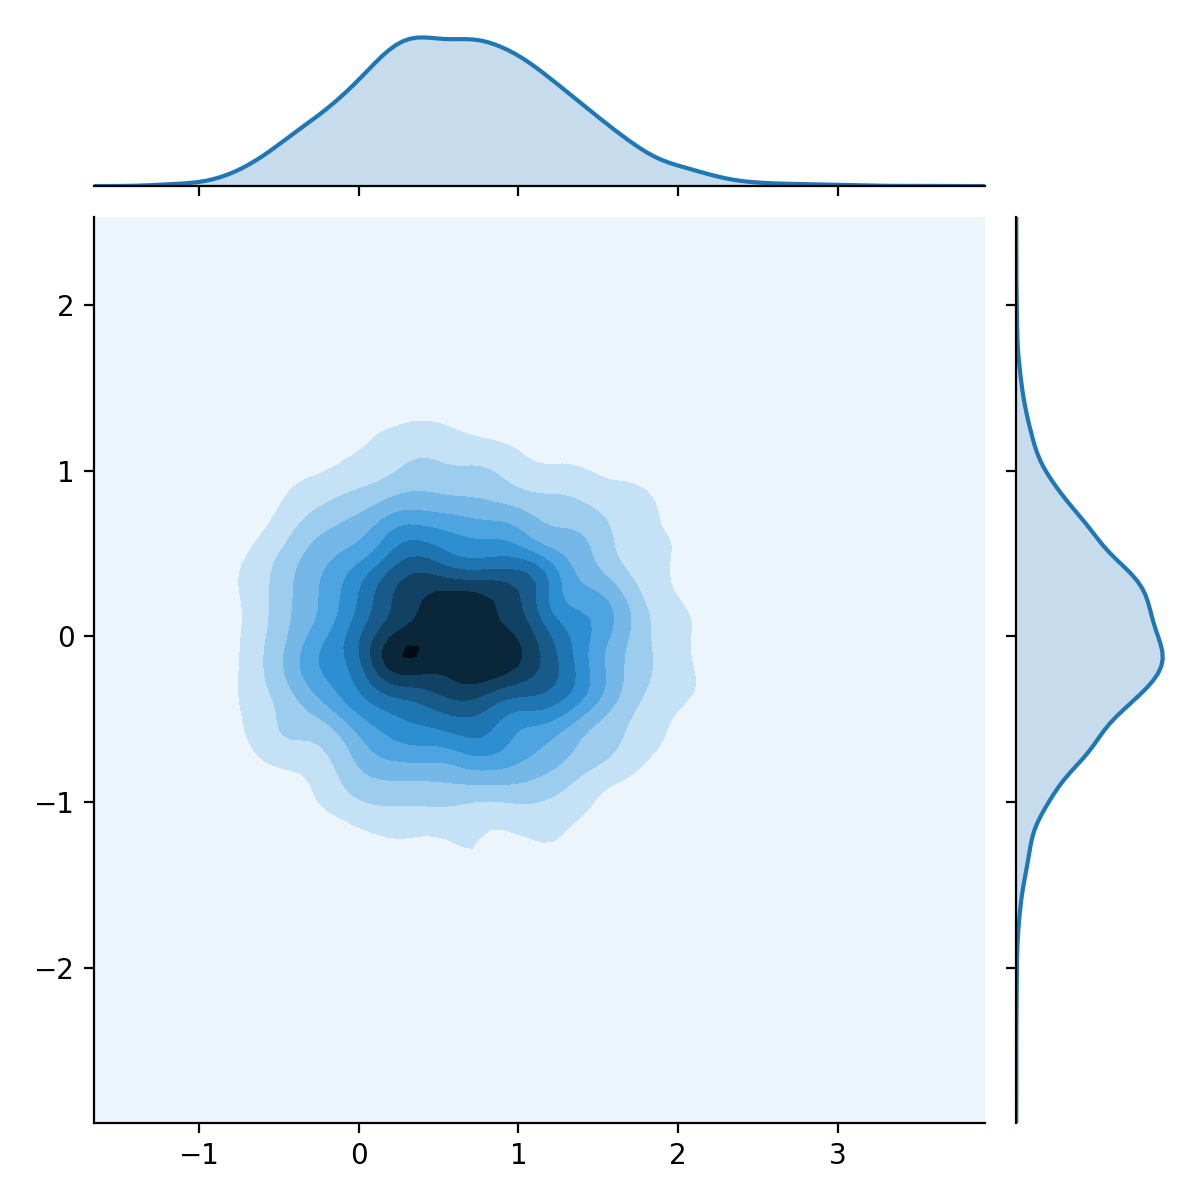
\includegraphics[scale=0.6]{figs/lasso_eg_samples.png}	
\caption{Posterior Sample KDE from MYULA. Sample mean at $(0.639, -0.019)^T$ with marginal variances of $0.44$ and $0.34$} 
\end{figure}



 
\newpage
\section{Total Variation Prior}



\newpage
\section{Wavelet Prior}

We can transform the image into a wavelet domain and penalise the coefficients in this new basis. Let $D$ be discrete wavelet transformation of an image $X$. We can transform the posterior to the wavelet domain:

\begin{equation}
	
\end{equation}






\newpage
\section{Smooth Input Convex Neural Networks}

The nodes of ICNNs are of the form:
\begin{align*}
 z_{i+1} = \phi_i ( B_i (z_i) + W_i(x_i) + b_i)	
\end{align*}
so if we use a smooth activation function $\phi_i = \text{softmax}$ we will have a smooth $g$, allowing us to ignore the prox step entirely. 















\end{document}
